\documentclass[a4paper]{article}

\usepackage[utf8]{inputenc}
\usepackage[english]{babel}
\usepackage{authblk}
\usepackage{adjustbox}
\usepackage{enumitem}
\usepackage{caption}
\usepackage{xfrac}
\usepackage[pdf]{graphviz}
\usepackage{pgf-umlsd}
\usepackage{array}
\usepackage{makecell}
\usepackage{booktabs}
\usepackage{xcolor}
\usepackage{amsmath}
\usepackage{amssymb}
\usepackage{mathtools}
\usepackage{listings}
\usepackage{verbatim}
\usepackage{indentfirst}
\usepackage[T1]{fontenc}
\usepackage[colorlinks=true, allcolors=blue]{hyperref}
%\usepackage[a4paper,top=3cm,bottom=2cm,left=3cm,right=3cm,marginparwidth=1.75cm]{geometry}

\babelhyphenation[english]{every-where}
\usetikzlibrary{shapes,arrows}

\newcolumntype{M}[1]{>{\raggedright\arraybackslash}m{#1}}

\lstdefinestyle{mystyle}{
    backgroundcolor=\color{lightgray}, 
    commentstyle=\color{codegreen},
    keywordstyle=\color{magenta},
    numberstyle=\tiny\color{lightgray},
    stringstyle=\color{codepurple},
    basicstyle=\footnotesize,
    breakatwhitespace=false,     
    breaklines=true,                 
    captionpos=b,                    
    keepspaces=true,                 
    numbers=left,                    
    numbersep=5pt,                  
    showspaces=false,                
    showstringspaces=false,
    showtabs=false,                  
    tabsize=2
}
\lstset{style=mystyle}
 
\providecommand{\tightlist}{%
  \setlength{\itemsep}{0pt}%
  \setlength{\parskip}{0pt}%
  \setlength{\topsep}{0pt}}

\title{\textsc{Prometheus}:\\Scalable High-load Computing \& Machine Learning on top of Bitcoin}
\author[1,2]{Maxim Orlovsky\thanks{orlovsky@pandoracore.com}}
\author[1,3]{Sabina Sachtachtinskagia\thanks{sabina.aueb@gmail.com}}
\affil[1]{Pandora Core AG, Switzerland}
\affil[2]{BICA Labs, Switzerland}
\affil[3]{Athens University of Economics and Business, Greece}

\date{Version 0.1.0, working draft}

\begin{document}

\maketitle

\begin{abstract}
This work defines Prometheus, a protocol for running high-load \& machine learning computing inside a trustless decentralized environment in Byzantine-tolerant way, utilizing bitcoin blockchain and script functionality, layer 2 state channels, zero knowledge computation integrity arguments, economic incentives and p2p networking.

This work covers questions of Prometheus design rationale, architecture, formal protocol  definition, transaction-based model and specifies protocol operations with demonstrable Nash equilibrium; the latter part is based on our previous work on incentive-based interactive settlement scheme for computation integrity proofs \cite{ibiss}.

This work will be followed by the papers on (1) specific probabilistically checkable proof schemes for high-load \& machine learning computing, addressing the problems of non-determinism in artificial neural networks, data privacy and federated learning and (2) underlying P2P communication protocol for global state replication and state channel management.
\end{abstract}


\section{Background \& Rationale}

The modern success of cloud computing is related to the economy of scale phenomenon, enhanced by the exponentially increasing amounts of produced data. However, it has created systematic risks and fragility, namely vanishing privacy, possibilities of totalitarian control, surveillance, single points of failure and censorship. It has put at risk the further development of machine learning technologies, which have started to be monopolised together with the access to big data. \href{https://manifesto.ai}{The \#FreeAI Manifesto} \cite{freeai} had declared an initiative to oppose this dramatic trend, and this work aims at the development of the technology stack able to address the issue.

The problem of censorship-resistant computing consists of many parts, starting from  finding and buying information (big data, machine learning models) in a censorship-resistant way, owning it with proper privacy and plausible deniability -- and up to computations using big data in anonymous and censorship-resistant and (desirably) private manner. Prometheus protocol addresses the latter issue, since the former two matters (finding and owning information) can be solved with many other existing initiatives, such as dark/anonymous markets, cryptography technologies, zero-knowledge, distributed storage and data transfer (Torrent, IPFS) etc \cite{ipfs, bittorrent, afs, tor, gnunet}. 

The actual technical problem we need to tackle in order to reach our goal is the proofs for computational integrity (correctness of the actual computations) for the computing performed by some non-trusted (anonymous) third parties -- without the need to repeat the whole volume of the actual computing. This issue is usually addressed by the use of probabilistically checkable proofs (PCP) -- however, they leave untouched the question of coupling the payments for the consumed computational resources with the actual proof. This question was resolved in our previous work \cite{ibiss}. 

Ability to run PCP schemes without trusted checking party provides a way to codify the actual protocol in terms of smart contracts, so it can be used in a very compact form with existing economic blockchain layer. Our approach to protocol design aims at the smallest possible size of the shared system state so it can be implemented with any non-Turing complete smart contract system with storing nothing else than the account balances (or UTXOs) and their un-locking conditions for the involved parties. For example, the protocol can be implemented with the existing Bitcoin script functionality with only two on-chain transactions per whole protocol computing cycle. In such system the PCP proofs are used at the second layer on top of slow blockchain, reducing the footprint, price and increasing scalability for the real-world business.

\section{Generic Protocol}

\subsection{Architecture}
\label{architecture}
A core of the protocol is based on the following main algorithms and cryptographic schemes:
\begin{description}
    \item[IBISS-CIP] Incentive-based interactive settlement scheme for computation integrity arguments: a game theory model for providing provably-safe economic incentives \cite{ibiss}
    \item[Bitcoin] including Bitcoin as a mean of payment, bitcoin blockchain as a safety and immutability layer, Bitcoin Script and HTLC smart contracts for the settlement algorithm logic.
    \item[PCP] probabilistically checkable proofs \cite{pcp, pcpibm} as non-interactive computation integrity verification technology
    \item[P2P Networking] for building decentralised network of nodes
\end{description}

The protocol is designed in a modular way, with four main components:
\begin{description}
    \item[Settlement algorithm] based on a game theory model with provable Nash equilibrium described in Section \ref{settlement} – an implementation of IBISS-CIP scheme \cite{ibiss}
    \item[Transaction model] defining set of interdependent off-chain and on-chain transactions with corresponding HLTV/CLTV/multisig smart contracts, described in Section \ref{transaction_model}
    \item[Networking protocol] for P2P node communications and information exchange
    \item[HLML-PCP schemes] PCP extension schemes for high-load computing and machine learning-specific tasks (HLML)
\end{description}

\begin{figure}[h!]
    \centering
    \begin{adjustbox}{center}\digraph[scale=0.75]{structs}{
        node[shape=record]
        prometheus [
            label="{
                {Prometheus protocol} 
                { <sa> Settlement algorithm & <sc> Transaction model & <zk> HLML-PCP schemes & <wp> Networking protocol} 
            }"
        ];
        bitcoin [label="Distributed ledger"];
        pcp [label="PCP"];
        ibiss [label="IBISS-CIP"];
        p2p [label="P2P networking"];
        
        prometheus:sc -> bitcoin;
        prometheus:zk -> pcp;
        prometheus:sa -> ibiss;
        prometheus:wp -> p2p;
    }\end{adjustbox}
    \caption{Architecture of the Prometheus protocol}
    \label{fig:architecture}
\end{figure}

Particularities of specific PCP gadgets for high-load \& machine learning computing, as well as P2P protocol are not covered by these document.

\subsection{Scopes and Actors}
\label{scopes_actors}

The protocol operates within two different scopes: \textbf{global scope} $\Gamma$ and \textbf{channel scope} $\Lambda$.

The protocol design includes the following types of participants (actors):
\begin{description}
    \item[Client node] $C$: party prepared to pay for the actual computing and provide necessary data for it.
    \item[Worker node] $W$: party prepared to perform actual computing for some reward.
    \item[Verifier node] $V$: party prepared to verify the actual computing using HLML-PCP.
    \item[Arbiter nodes] $\mathbb{A}$ (global) and their subset $\mathcal{A}$ (for a given computing contract): a special sets of nodes committed to do the arbitration work
    \item[Common fund] $F$: used as a wild card destination for penalty payments. This can be a deterministic unspendable contract, or a special contact for funding protocol development etc. The particular value form of common fund is defined by each of Prometheus contracts (see below).
\end{description}

Clients, Workers and Verifiers (as well as the common funds) operate only within \textit{channel scope}, while Arbiters are defined within the \textit{global scope} (denoted by $\mathbb{A} \mid \Gamma$) and are able to participate in \textit{channel scope} (denoted by $\mathcal{A} \mid \Lambda$).

\subsection{Layers, Contracts and States}
\label{layers_contracts}

The protocol operates using different layers of abstraction, each of which contains its own set of contracts:
\begin{enumerate}
    \item \textbf{Global consensus state} $\mathsf{G} \mid \Gamma$ based on blockchain-stored state $\Gamma^\Omega$ and off-chain data $\Gamma^\Theta$, committed to the blockchain with hashes and replicated by all parties participating the protocol:
    \begin{description}
        \item[Prometheus contracts] $\{ \mathsf{P}_i \} \mid \Gamma$: specially-formed contracts encoding pre-defined sets of global parameters. These are \textit{commitment-based agreement}, i.e. agreements that can be referenced by any independent party as a commitment to follow/accept these pre-defined values. Basically, it is a tuple of meta-parameters:
        
        $\mathsf{P} = \langle w, v, n, a, F, \alpha, \beta,  \gamma, \delta, \varepsilon, \mu, \sigma, t_1, t_2, t_3, t_4 \rangle$ 
        
        For the meaning of the constants see Table~\ref{table:state}.
        
        \item[Arbitration offers] $\{ \mathsf{O}_i \} \mid \Gamma$: specially-formed contracts from parties that want to act as Arbiters in any future computation contract. These contracts are committed to particular Prometheus contract $\mathsf{P}_i$ and must contain proofs of the locked arbiter's stake of size $a$ (defined by $\mathsf{P}_i$): $\mathsf{O} = \langle \mathsf{P}_i, a_p \rangle$. Parties that have made these commitments constitutes global set $\mathbb{A}$.
        
        \item[Computational contracts] $\{ \mathsf{C}_i \} \mid (\Gamma \vee \Lambda)$: \textit{economically-binding agreements} committed to some particular contract $\mathsf{P}_i$ between parties $C, W, V$ containing proofs of their locked stakes $w_p,v_p$ (corresponding to the amounts defined by $\mathsf{P}_i$), computational reward $c$ and computation-related $\mathtt{payload}$: $\mathsf{C} = \langle \mathsf{P}_i, C, W, V, c, w_p, v_p, \mathtt{payload} \rangle$. Computational contract locks deposits and includes all possible settlement schemes (see Table 2).
        
        \item[Arbitration contracts] $\{ \mathsf{A}_i \} \mid (\Gamma \vee \Lambda)$: \textit{economically-binding agreements}  committed to some particular contract $\mathsf{C}_i$ by Arbiters (denoted as $\mathcal{A}$) that were randomly selected from $\mathbb{A}$ to participate in Arbitration stage of the computing contract. The contract contains proofs of the arbiter's stake commitments ($a_p$): $\mathsf{A} = \langle \mathsf{C}_i, \mathcal{A}, \{ a_{p_i} \mid \forall A_i \in \mathcal{A} \} \rangle$
    \end{description}
    
    \item \textbf{Multiparty state channel} $\mathsf{M}(\mathsf{C}_i) \mid \Lambda$ originating from each computational contract $\mathsf{C_i}$: $\mathsf{M}(\mathsf{C}_i) = \langle \mathsf{C_i}, \Upsilon, \pi, \mathtt{Encrypt}(\Pi, h_p)\rangle$. The channel operates the following state data:
    \begin{description}
        \item[Partially-signed transaction tree] $\Upsilon$, which defines:
        \begin{itemize}
            \item Current \textbf{operational state} of the channel (see below for the details);
            \item \textbf{Hash-lock value} $h$ provided by the Worker and used in hash-locked transactions within $\Upsilon$ to bind the use of reward $c$ by the Worker with the ability of the Client to read the results of computation, encrypted with this hash \textit{preimage} $h_p$ (see below);
            \item \textbf{Verifier's verdict} $r=\{\emptyset,0,1\}$ on Worker's proofs of computational integrity. Verdict equals to $\emptyset$ before the completion of the Verification phase (see below);
            \item \textbf{Set of Arbiters} $\mathcal{A}$ (equals to $\emptyset$ befor the start of arbitration phase);
            \item \textbf{State of arbitration contract} $\mathsf{A}_i$ and corresponding signed but unpublished transactions
            \item \textbf{Arbitration decision} $d=\{\emptyset,0,1\}$: \textit{economically-binding decision} provided by $\mathcal{A^+}$ (subset of $\mathcal{A}$ which have signed to the decision). Equals to $\emptyset$ before the completion of arbitration phase -- or in case if no definite decision was reached.
        \end{itemize}
        \item[Non-interactive probabilistic proofs] $\pi$ of computational integrity provided by the Worker at the end of computation phase.
        \item[Computation results] $\Pi$ encrypted with \textit{preimage} $h_p$ by the Worker.
    \end{description}
    
    \item \textbf{Internal state} of the actors ($C, W, V, A_i$): each party acts as a part of channel state machine (i.e. it is replicated \& semi-synchroneous state machine). Thus, the internal state  of the party is tightly related to the state of the channel (see below). When required, the current state of the party is denoted with  precondition notation: for instance, $W\mid \Lambda^\mathsf{C}$ represents Worker node under computing state, while $\Lambda^\mathsf{C} \mid\: W$ represents channel in computing state with Worker node signed confirmation (agreement) on the state published into the channel.
\end{enumerate}

For the complete list of state parameters see Table~\ref{table:state}.

\begin{table}[hp]
    \caption{Summary of state parameters}
    \label{table:state}
    \begin{adjustbox}{center}
        \begin{tabular}{@{} l m{11cm} m{2.5cm} c @{}}
            \toprule
            Parameter & Description & Bounding\-conditions & Defined by \\
            \midrule
&\textbf{1. Actors, signatures and stakes} \\
            $W, V, C$ & Worker, Verifier and Client as actors identified by their signatures & $W \ne V \ne C$ & $\mathsf{C}$ \\
            $w, v$ & Stakes deposited by Worker and Verifier & \makecell{$w \gg z$, $v \gg y$,\\ $w \le v$} & $\mathsf{P}$ \\
            $c$ & Amount the Client is willing to pay for the computation & $c \gg z \gg y$ & $\mathsf{C}$ \\
            $z$ & Cost incurred by the Worker for performing the computation & $z \ll c$ & $W$ \\
            $y$ & Cost incurred by the Verifier for performing the verification & $y \ll z \ll c$ & $V$ \\
            $F$ & \textit{Common fund} public key/address which is controlled by external body (can be charity, donations to development, deterministic proof of burn address or anything else) & & $\mathsf{P}$ \\
            $\mathbb{A}$ & Global set of pre-registered Arbiters & $\mathbb{A} \ne \emptyset$ & $\mathsf{O}$ \\
            $\mathcal{A} = \{A_i\}$ & Set of randomly-selected Arbiters as actors identified by their signatures & $\mathcal{A} \subset \mathbb{A}$ $\mid\mathcal{A}\mid\: \ge 3$ & $\mathsf{M}$ \\
            $\mathcal{A^+}$ & Subset of Arbiters that have made a coherent decision & $\mathcal{A^+} \subset \mathcal{A}$ & $\mathsf{M}$ \\
            $\mathcal{A^-}$ & Subset of Arbiters that didn't participate or agreed with a coherent decision & \makecell{$\mathcal{A^-} = \mathcal{A} \setminus \mathcal{A^+}$ \\ $\mathcal{A} = \mathcal{A^+} \cup \mathcal{A^-}$ \\ $\mid\mathcal{A^+}\mid\; > \mu \mid\mathcal{A^-}\mid$} & $\mathsf{M}$ \\
            $n$ & Size of $\mathcal{A}$ (amount of Arbiters participating arbitration) & $3 \le n \ll\: \mid\mathbb{A}\:\mid$ & $\mathsf{P}$ \\
            $a$ & Standard stake of Arbiter locked in blockchain-based contract & $a \gg v$ & $\mathsf{P}$ \\
            \midrule
&\textbf{2. Cryptographic functions and arguments}\\
            $h, h_p$ & Hashed value $h$ and its \textit{preimage} $h_p$ initially selected and known only to the Worker. $h_p$ is used to encrypt the content of the data file. & $h = \mathtt{HASH}(h_p)$ & $W$ \\
            $t_1, t_2, t_3, t_4$ & \textit{Timelock} conditions ordered in such a way that smaller-indexed timelock precedes in time timelocks with larger indexes & $t_i \prec t_{i+n}$ & $\mathsf{P}$ \\
            $T^k_n$ & $k$-of-$n$ threshold multisignature & $n = \mid\mathcal{A}\mid, k = \lceil \mu n\rceil$ & $\mathsf{M}$ \\
            $d$ & \textit{Decision} taken by Arbiters, such as $\mid d=1$ is a pre-condition satisfying that the \textit{voting majority} of Arbiters $\mathcal{A^+}$ found Worker $W$ of being faulty. & $d \in \{0, 1\}$ & $\mathsf{M}$ \\
            \midrule
&\textbf{3. Meta-parameters}\\
            $\alpha$ & Fraction of stake taken from Worker's deposit $w$ in case of its timeout & $0 < \alpha \le 1$ & $\mathsf{P}$ \\
            $\beta$ & Fraction of stake taken from Verifier's deposit $v$ in case of its timeout & $0 < \beta \le 1$ & $\mathsf{P}$ \\
            $\gamma$ & Fraction of Worker's stake $w$ that is awarded to the Client as a compensation payment in case the Arbitation was not being able to reach a final decision & $0 < \gamma < \varepsilon$ & $\mathsf{P}$ \\
            $\delta$ & Fraction of stake $w$ taken from Worker $W$ if it was found faulty by the Verifier and didn't appeal & $\delta \le w-(1-\sigma)c$ & $\mathsf{P}$ \\
            $\varepsilon$ & Fraction of stakes that all participants ($W, V, \mathcal{A}$) are penalised in case of failed Arbitration (i.e. when $\mid\mathcal{A^+}\mid\; < \mu \mid\mathcal{A}\mid$) & $\gamma < \varepsilon \le 1$ & $\mathsf{P}$ \\
            $\mu$ & \textit{Arbiter voting majority}: threshold for Arbiters decision making & $\mu > 0.5$ & $\mathsf{P}$ \\
            $\sigma$ & Fraction of computation used by Worker in its \textit{computation argument} -- and subsequently verified by Verifier. It also defines the proportion of Client's payment $c$ that goes to Worker $W$ in case of successful computing (correspondingly, Verifier $V$ will receive reward of $1-\sigma c$) & $0 \le \sigma \le 1$ & $\mathsf{P}$ \\
            \bottomrule
        \end{tabular}
    \end{adjustbox}
\end{table}

Multiparty state channel operates as a deterministic finite state machine with the following possible states (see also Fig.~\ref{fig:states}):
\begin{description}
    \item[Setup] $\Lambda^\mathsf{S}$, performed by all parties interactively
    \item[Computation] $\Lambda^\mathsf{C}$, performed by Worker
    \item[Verification] $\Lambda^\mathsf{V}$, performed by Verifier
    \item[Arbitration] $\Lambda^\mathsf{A}$ (optional phase), performed by special group of Arbiters
    \item[Closed] $\Lambda^\mathsf{\times}$ with one of the settlement schemes published to the global state $\mathsf{G}$ (for settlement schemes see next section and Table~\ref{table:settlement}). The used settlement scheme is denoted in the subscript of the channel state, i.e. $\Lambda^\mathsf{\times}_\mathtt{3}$.
\end{description}

State transitions are denoted by arrows with state transition conditions listed above the arrow.

The normal state transition path is defined by $\Lambda^\mathsf{S} \xrightarrow{\mathsf{C}} \Lambda^\mathsf{C} \xrightarrow{\pi} \Lambda^\mathsf{V} \xrightarrow{r=1} \Lambda^\mathsf{\times}_\mathtt{3}$.

\begin{figure}[h!]
    \centering
    \begin{adjustbox}{center}\digraph[scale=0.75]{statemachine}{
        rankdir=LR; rank=same;
        { rank=same;
        setup -> computing;
        computing -> verification [label="proofs"];
        verification -> closed [label="verdict"]; }
        setup -> closed [style=dotted, label="no agreement"];
        computing -> closed [style=dotted, label="timeout"];
        verification -> arbitration [label="appeal"];
        arbitration -> closed [label="decision"];
    }\end{adjustbox}
    \caption{Possible channel states and transitions}
    \label{fig:states}
\end{figure}

\section{Settlement Algorithm}
\label{settlement}

Prometheus \textit{settlement algorithm} provides economic incentives and settlement schemes with a provable Nash equilibrium for non-Byzantine behaviour of all of the rational participants. It is developed on top of incentive-based interactive settlement scheme for computation integrity proofs \cite{ibiss}.

The algorithm runs in five phases (Fig.~\ref{fig:states}), each of which corresponds to particular state of the channel (Fig.~\ref{fig:states})

\begin{figure}[hp]
    \centering
    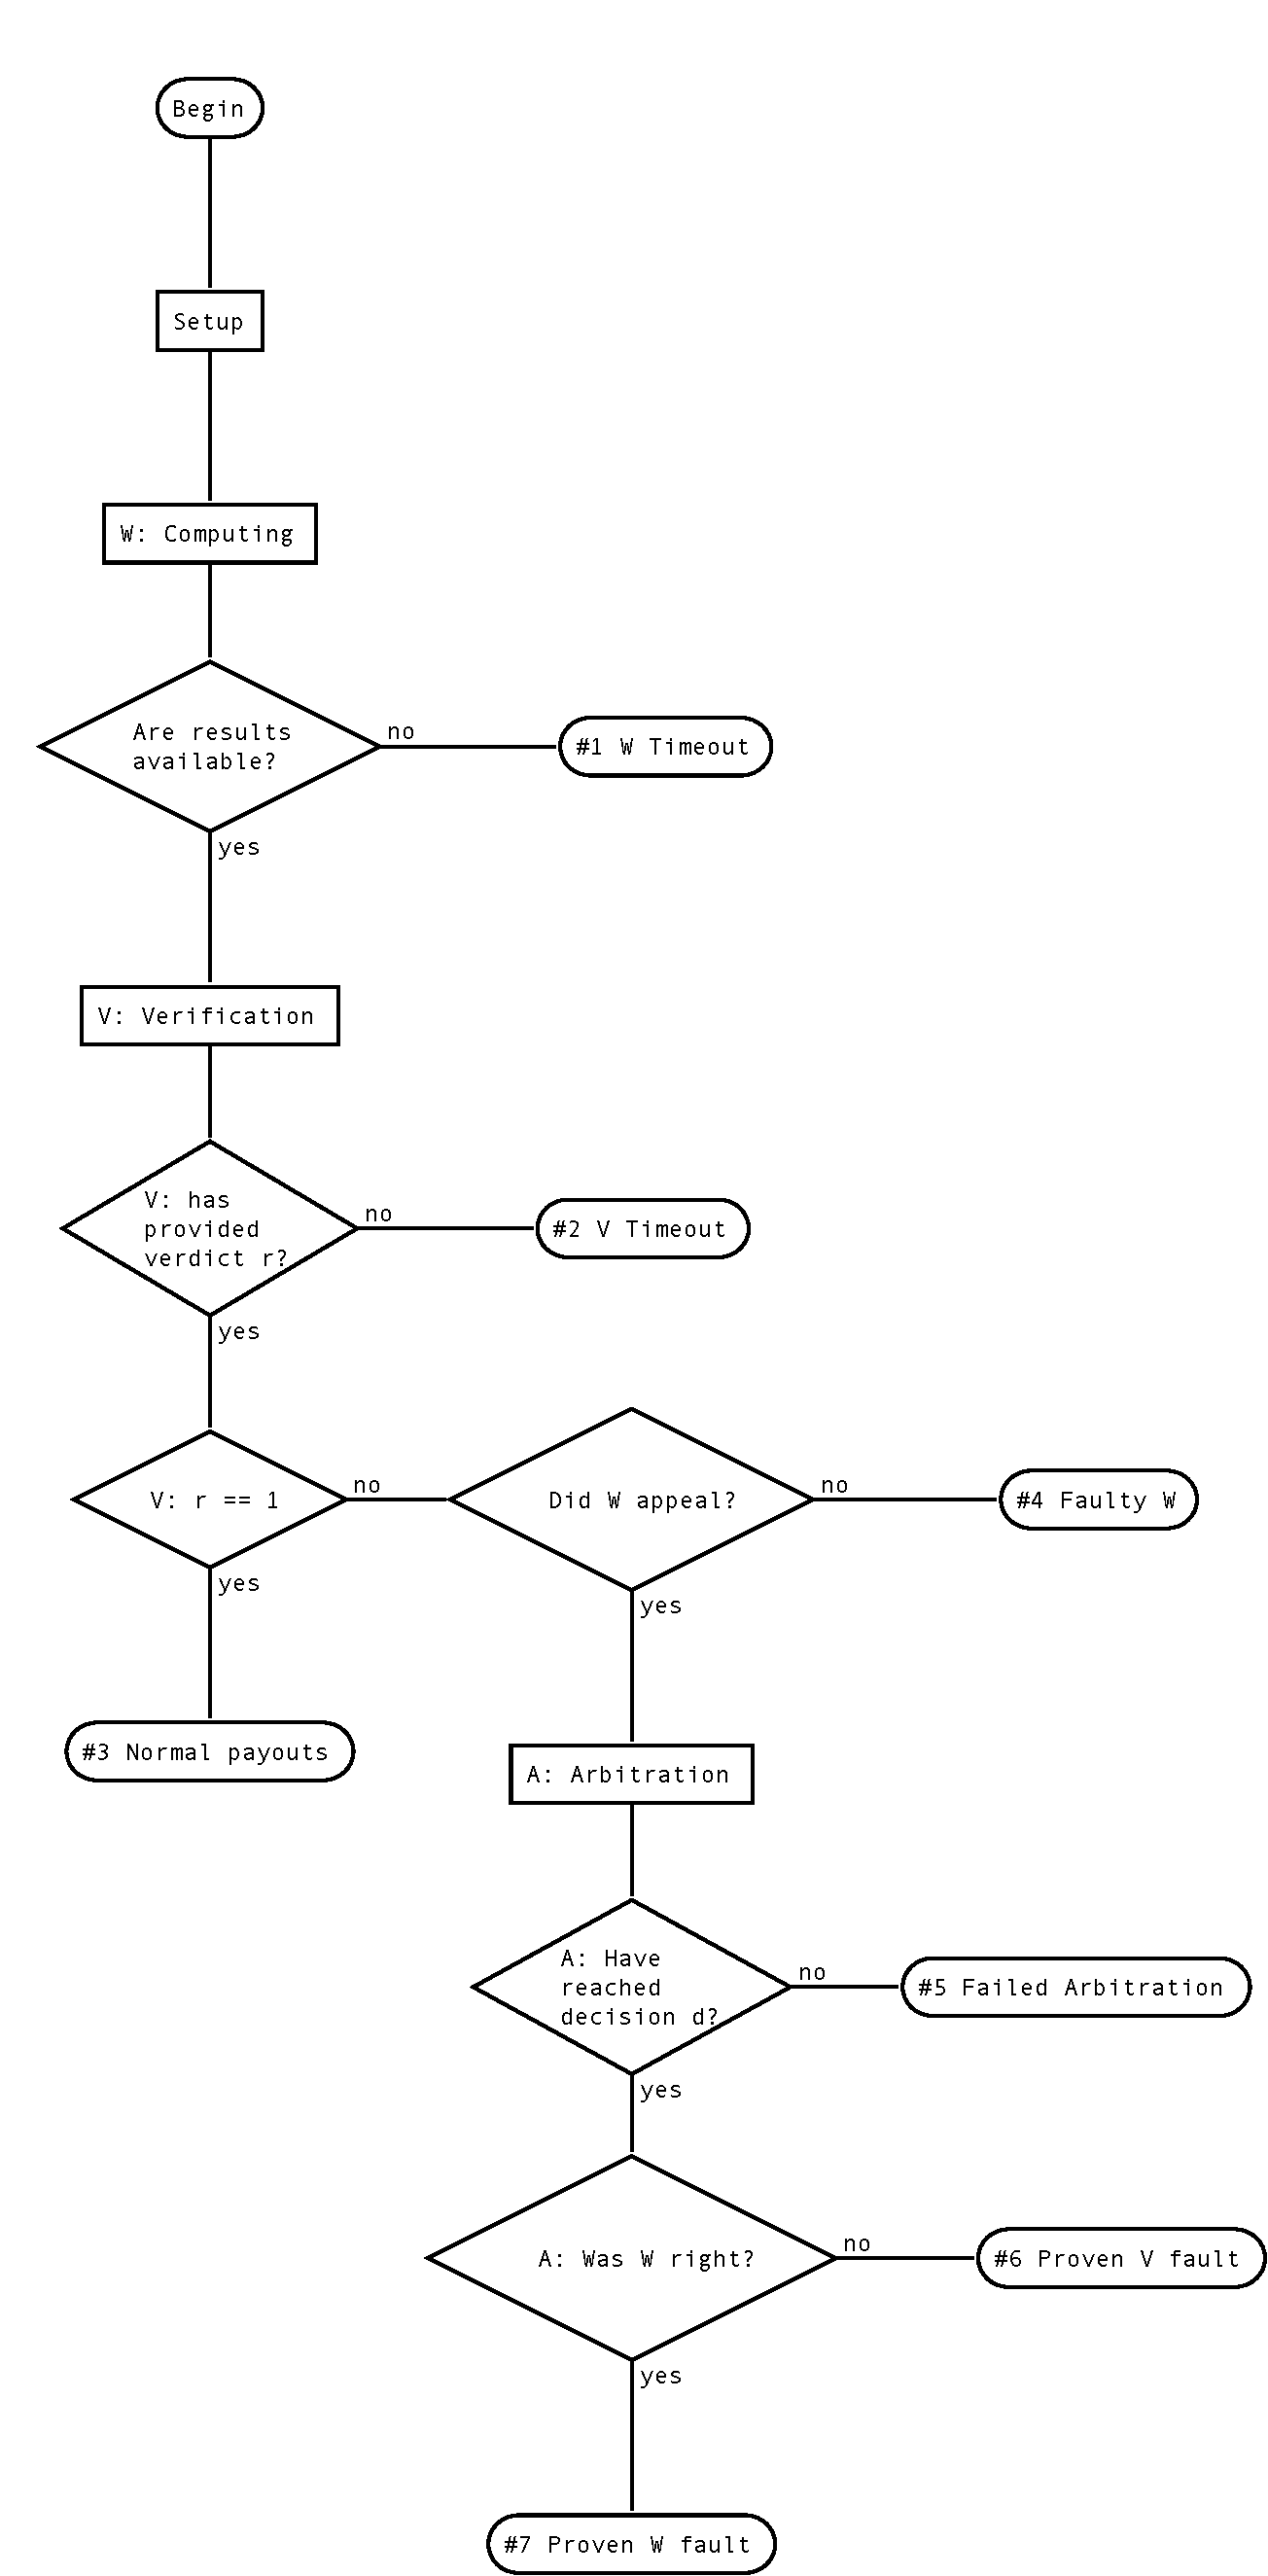
\includegraphics[height=1.5\columnwidth]{assets/settlementflow.pdf}
    \caption{Prometheus settlement algorithm flowchart}
    \caption*{\textit{Rectangles corresponds to contract phases and channel states; numbered exists (\#1, \#2 etc) corresponds to the settlement schemes from the Table~\ref{table:settlement}}}
    \label{fig:settlementflow}
\end{figure}

\subsection{Algorithm phases}
\label{phases}

\subsubsection{Setup -- $\Lambda^\mathsf{S}$}
During the Setup phase, the Client node splits the actual computing task into \textit{batches} suitable for parallel processing in a distributed P2P network.

For each batch, the client selects Worker and Verifier nodes on some open market or by auction (the actual selection is not part of this protocol). They agree upon the contract conditions (by committing to particular Prometheus contract $\mathsf{P}_i$) and computation reward $c$ in the process of off-chain P2P communications. 

To secure the actual contract Client, Worker and Verifier put $c, w, v$ under the \textit{computation contract} as described in section \ref{layers_contracts} and publish it to the blockchain.

\subsubsection{Computation -- $\Lambda^\mathsf{C}$}
Worker node downloads all necessary data according to the contract and runs actual computation. Upon their completement the Worker encrypts the results with $h_p$ value, prepares PCP proof $\pi$ with one of the HLML-PCP schemes and updates the state of the channel with these data. The proof is constructed for some pre-defined portion of the data $\sigma$.

If the phase is not completed within the pre-defined time, the Client or the Verifier has the right to terminate the contract and penalise the Worker (see settlement scheme \#1 in Fig.~\ref{fig:settlementflow} and Table~\ref{table:settlement})

\subsubsection{Verification -- $\Lambda^\mathsf{V}$}
Verifier node downloads source data with proofs $\pi$, checks them and reports \textit{verdict} $r$ into the channel. If the Worker found faulty, it has the right to either \textit{appeal} and start Arbitration procedure -- or \textit{admit the fault} by signing another transaction corresponding to settlement scheme \#4 (see Table~\ref{table:settlement}). In this case Worker will have a smaller penalty and we will prevent unnecessary computation load.

If the phase is not completed within the pre-defined time, the Worker has the right to terminate the contract and penalise Verifier (see settlement scheme \#2 in Fig.~\ref{fig:settlementflow} and Table~\ref{table:settlement})

\subsubsection{Arbitration -- $\Lambda^\mathsf{A}$}
Arbiters $\mathcal{A}$ participating the Arbitration phase of the particular computing contract must be chosen from the global arbiters pool/set $\mathbb{A}$ (established well before the initiation of the computing contract) with some deterministic randomness procedure. This is required in order to prevent actors of spamming the Arbiters pool with their agents once the contract has reached Arbitration stage. 

Before become part of the $\mathcal{A}$ each of the selected Arbiters must confirm their participation via off-chain messaging. Jointly Arbiters constituting $\mathcal{A}$ sign their stakes into the computing contract with economically binding contract $\mathsf{A}$ as described in section \ref{layers_contracts} above.

Arbiters reach decision in process of independent checks of $\pi$ proofs and P2P communications. To reach decision at least $\mu$ part of all Arbiters must come to the same coherent conclusion, where $\mu$ is a so-called \textit{voting majority} -- a parameter defined by Prometheus contract $\mathsf{P}_i$.

If Arbiters are unable to reach a \textit{coherent decision} ($d=\emptyset$) with $\mu\%$ of votes, the computing contract defaults to payment scheme \#5 (Table~\ref{table:settlement}) where all of the contract participants (except of the Client) are penalised and the Client is compensated with some slice of their stake.

If the coherent decision has being made, the contract completes with either \#6 or \#7 payment schemes (Table~\ref{table:settlement}) depending on the decision. In both schemes, the parties found faulty are penalised; and it the Worker computation results are found correct, the Worker receives its payment and the Client is provided with the results.

\subsubsection{Payouts and Channel Closing -- $\Lambda^\mathsf{\times}$}
Depending on the completion of the phases 2, 3 and 4 there might be different ways of the final settlement, numbered on the Fig.~\ref{fig:settlementflow} from \#1 to \#7 and described below in the Table~\ref{table:settlement}.

The channel is closed by publishing the singed branch of the transaction tree $\Upsilon$ from the channel scope into the global scope: $\Lambda^{\times} \xrightarrow{\Upsilon} \Gamma$.

In cases when the computations by the Worker were proven to be correct (schemes \#2, \#3 and \#7) in order to take its reward the Worker must publish to the blockchain a spending transaction containing \textit{preimage} $h_p$ used for encrypting the resulting data payload~-- thus allowing Client to read its value and decrypt the data.

\begin{table}[h!]
    \caption{Settlement schemes}
    \label{table:settlement}
    \begin{adjustbox}{center}
        \begin{tabular}{@{} l m{2.5cm} m{5cm} m{3cm} l @{}}
            \toprule
            ID & Scheme & Payout schedule & \makecell[l]{Precondition\\ $\mid$ postcondition\footnotemark[1],\footnotemark[2]} & Deposit redistribution\footnotemark[1] \\
            \midrule
            \#1 & Worker timeout & Penalise Worker with a fraction of stake 
            & \makecell[l]{$\ldots \Lambda^\mathsf{C} \xrightarrow{\pi=\emptyset}$\\ $\mid\: t_3 \wedge (C \vee V)$ }
            & $W: -\alpha w \rightarrow F$ \\
            \midrule
            \#2 & Verifier timeout & Pay to Worker, penalise Verifier with a fraction of stake to Client 
            & \makecell[l]{$\ldots \Lambda^\mathsf{V} \xrightarrow{r=\emptyset}$\\ $\mid\: t_1 \wedge W \wedge h_p$ }
            & \makecell[l]{$V: -\beta v \rightarrow C,$\\$C: -\sigma c \rightarrow W$} \\
            \midrule
            \#3 & Normal payouts & Pay to Worker and Verifier 
            & \makecell[l]{$\ldots \Lambda^\mathsf{V} \xrightarrow{r=1}$\\ $\mid\: W \wedge h_p \wedge V$ }
            & \makecell[l]{$C: -\sigma c \rightarrow W,$\\$C: -(1-\sigma) c \rightarrow V$} \\
            \midrule
            \#4 & Faulty Worker, no appeal & Pay to Verifier from Worker stake, penalise Worker with a fraction of stake 
            & \makecell[l]{$\ldots \Lambda^\mathsf{V} \xrightarrow{r=0}$\\ $\mid\: t_2 \wedge V \wedge W$ }
            & \makecell[l]{$W: -(1-\sigma)c \rightarrow V,$\\$W: -\delta w - (1 - \sigma)c$\\$\: \rightarrow F$} \\
            \midrule
            \#5 & Failed Arbitration (no coherent decision) & Penalise all participants, compensate Client 
            & \makecell[l]{$\ldots \Lambda^\mathsf{V} \xrightarrow{r=0} \Lambda^\mathsf{A} \xrightarrow{d=\emptyset}$\\ $\mid\: t_4 \wedge C$ }
            & \makecell[l]{$W: -\gamma w \rightarrow C,$\\ $W, V, \mathcal{A}:$\\$\: -\varepsilon(w+v+\sum a) \rightarrow F$} \\
            \midrule
            \#6 & Arbitration proved Worker fault & Penalise Worker with full stake transferred to Arbiters, penalise faulty Arbiters 
            & \makecell[l]{$\ldots \Lambda^\mathsf{V} \xrightarrow{r=0} \Lambda^\mathsf{A} \xrightarrow{d=1}$\\ $\mid\: T^k_n(\mathcal{A^+})$ }
            & \makecell[l]{$W: -w \rightarrow \mathcal{A^+},$ \\ $\forall A_i \in \mathcal{A^-}: -a_i \rightarrow F$} \\
            \midrule
            \#7 & Arbitration proved Verifier fault & Pay to Worker, penalise Verifier with full stake transferred to Arbiters and Fund, penalise faulty Arbiters 
            & \makecell[l]{$\ldots \Lambda^\mathsf{V} \xrightarrow{r=0} \Lambda^\mathsf{A} \xrightarrow{d=0}$\\ $\mid\: T^k_n(\mathcal{A^+}) \wedge W \wedge h_p$ }
            & \makecell[l]{$C: -c \rightarrow W$\\$V: -w \rightarrow \mathcal{A^+},$\\ $V: -(v-w) \rightarrow F,$\\ $\forall A_i \in \mathcal{A^-}: -a_i \rightarrow F$} \\
            \bottomrule
        \end{tabular}
    \end{adjustbox}
\end{table}
\footnotetext[1]{See Table~\ref{table:state} for the summary of the used state parameters}
\footnotetext[2]{The precondition is defined as a postfix of the state transition path in a part that is different from the normal state transition path $\Lambda^\mathsf{S} \xrightarrow{\mathsf{C}} \Lambda^\mathsf{C} \xrightarrow{\pi} \Lambda^\mathsf{V} \xrightarrow{r=1}$. 
The postcondition is a set of conditions which have to be satisfied by the computing channel state $\mathsf{M}$.}

\subsection{Game mechanics}
\label{game}

To analyse all possible game strategies we need to pay special attention to the timelock postconditions $t_1-t_4$. In fact, their existence splits the whole game into separate timeslots, within which only designated players have ability to "move" (i.e. to sign some particular version of payout scheme or to wait/default/pass move by timeout to the players of the next timeslot). The analysis of this moves and timeslots is given in the Fig.~\ref{fig:strategies}.

\begin{figure}[h!]
    \centering
    \begin{adjustbox}{center}
    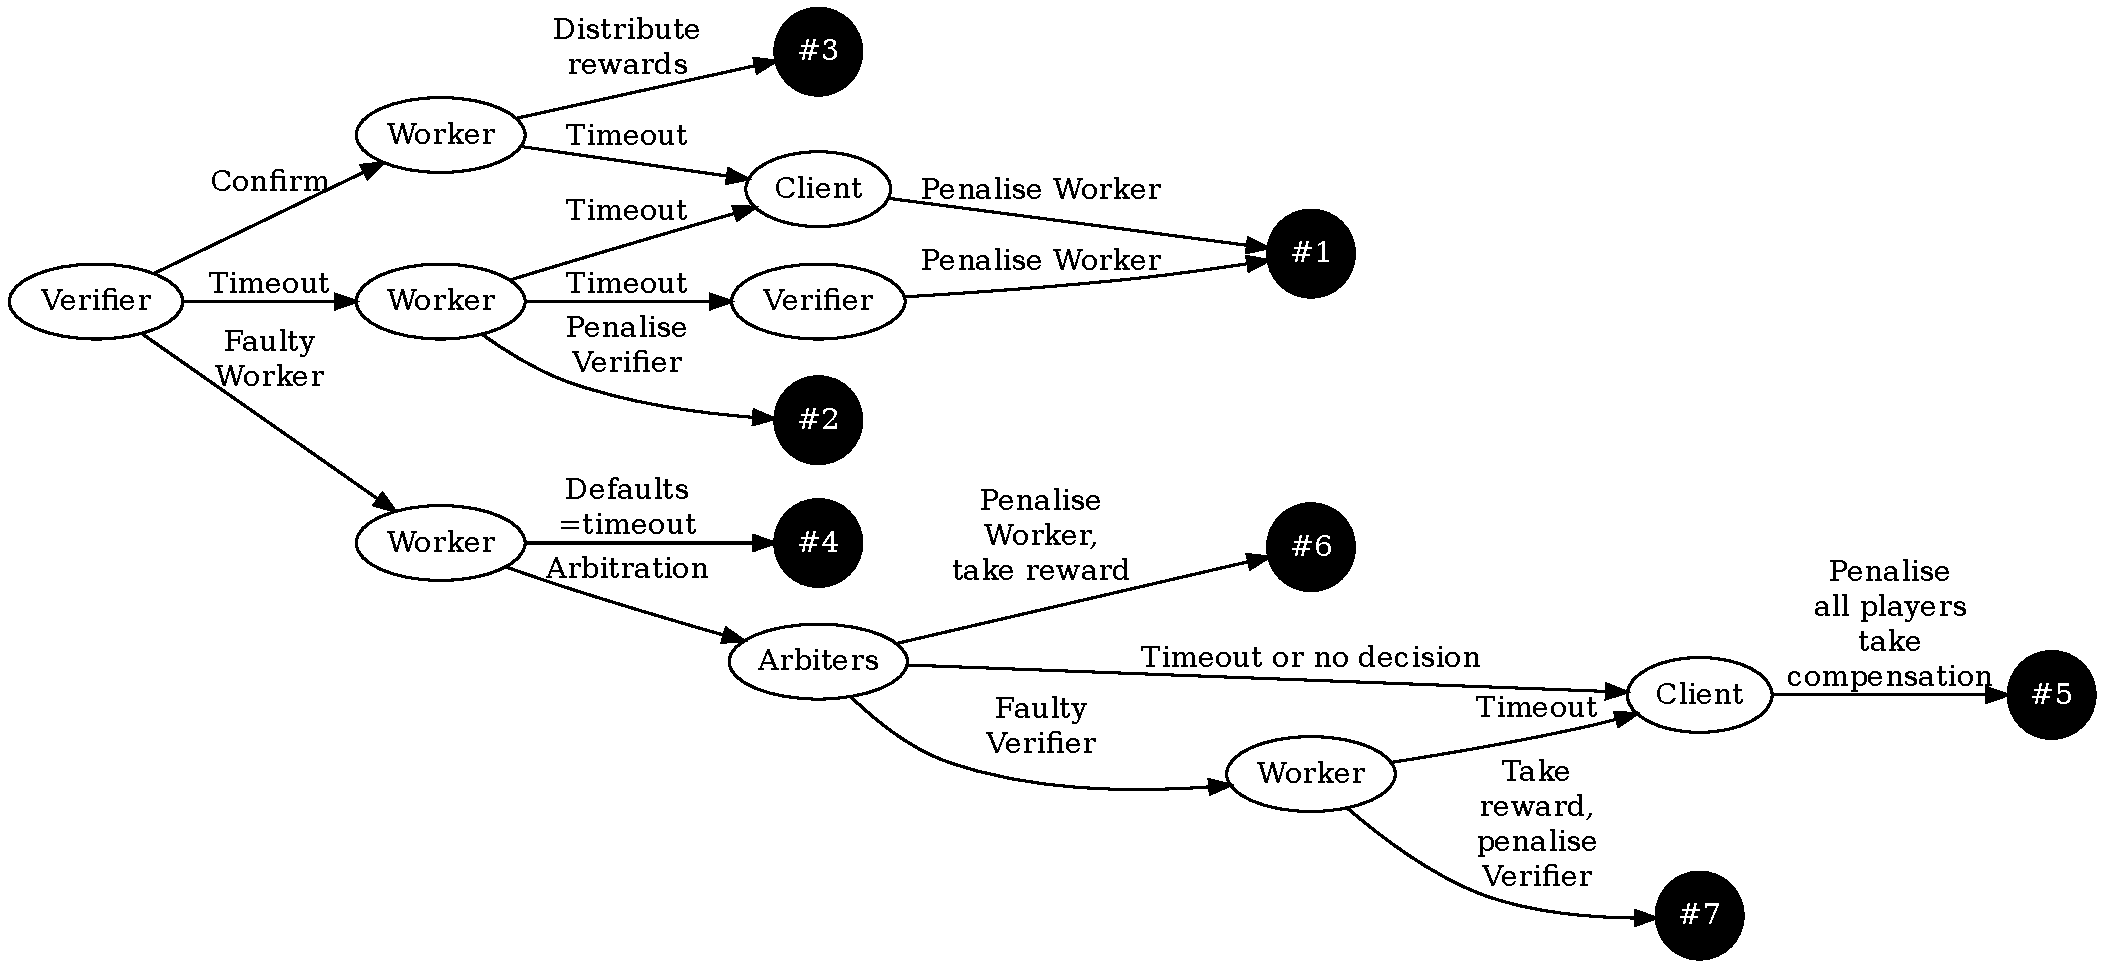
\includegraphics[width=1.2\columnwidth]{assets/strategies.pdf}
    \end{adjustbox}
    \caption{Possible game strategies}
    \label{fig:strategies}
\end{figure}

At the start of the game (setup phase), a complete set of seven possible payout transactions spending the deposited reward and stakes is created. Each of the transactions is pre-signed by all actors that are \textbf{not} present on the path leading to the settlement scheme corresponding to the transaction. Through the process of game each participant decides which transaction to sign and, by doing so, it adds to the post-condition criteria for the corresponding settlement scheme from the Table~\ref{table:settlement} -- until the completion and publication of one of them. Each signature on the path is equal to the change in the state of the channel and each game end-leaf (exit) is an implementation of some particular payout scheme.

Thus, by analysing both finite state machine and game theory models we have shown deterministic nature of the settlement algorithm leading to the Byzantine tolerance for the rational set of participants resulting in verified computation and proper reward distribution.

\section{Transaction model}
\label{transaction_model}

\subsection{Prometheus contracts}
\label{p_contracts}

Prometheus contracts $\{\mathsf{P}_i\}$ are defined in the global scope using on-chain transactions $\{ \mathsf{T}_{\mathsf{P}_i} \} \mid\Gamma^\Omega$. Each transaction stores a tuple of contract parameters $\mathsf{P} = \langle w, v, n, a, F, \alpha, \beta,  \gamma, \delta, \varepsilon, \mu, \sigma, t_1, t_2, t_3, t_4 \rangle$ in explicit form as part of its single \texttt{OP\_RETURN} output. Explicit storage is required for faster achievement of global state $\mathsf{G}$ syncronisation without requirements to run multiple P2P requests and data keeping. The cost of on-chain storage is low, since each of the Prometheus contracts will define some set of parameters matching well-known best practice and there are just few possible options that can satisfy conditions for the Nash equilibrium.

Prometheus contracts are committed to by arbitration offer and computational contract originating transactions by their transaction hash (\texttt{txid}, see sections below for the details).

\subsection{Arbitration offers}
\label{o_contracts}

Arbitration offers are contracts created by the parties wishing to participate in the future Arbitrations started by Worker appeals under computational contracts (see section Arbitration below).

Arbitration offer $\mathsf{O}_i$ by a party $A_i$ consists of a commitment to a particular Prometheus contract $\mathsf{P}_x$ and stake proof $a_p$ that corresponds by its value to the parameter $a$ withing the committed contract: $\mathsf{O} = \langle \mathsf{P}_x, a_p \rangle$. This information is packed into a transaction $\mathsf{T_O}$ with $a_p$ amount stored under HTLC P2SH contract in \texttt{scriptPubKey} of its first output and with second output referencing corresponding $\mathsf{T}_{\mathsf{P}_x}$ \texttt{txid} via \texttt{OP\_RETURN}  code (see Fig.~\ref{fig:txo}). HTLC type of the contract for the stake lock is required to protect from lateral stake spending during the \textit{computational contract} execution (see \ref{lifecycle} below) and from committing to multiple \textit{computational contracts}.

The purposes of such transaction is to:
\begin{itemize}[topsep=0pt]
    \tightlist
    \item Put information into the global state $\mathsf{G}$ about party willing to arbitrate under some specific contract conditions
    \item Prove availability of the funds required for creation of arbitration stake
    \item Prove time of the arbitration offer (important for achieving Nash equilibrium for the Prometheus settlement algorithms)
\end{itemize}

\begin{figure}[h!]
    \centering
    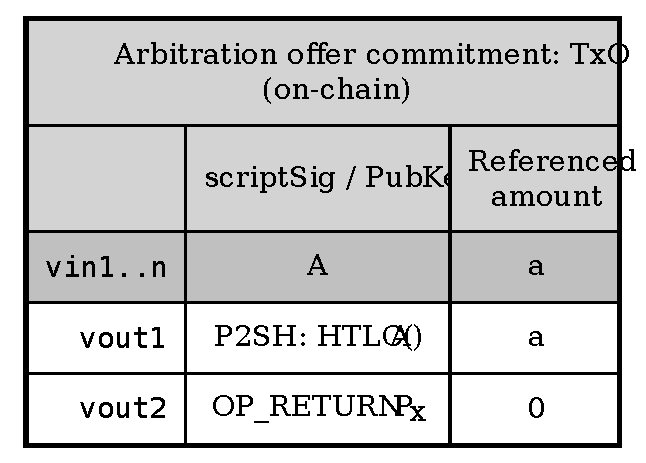
\includegraphics[scale=0.75]{assets/txo.pdf}
    \caption{Structure of the arbitration offer commitment transaction $\mathsf{T_O}$}
    \label{fig:txo}
\end{figure}

Only well-formed transactions with unspent output are taken as a part of global state of the system: $(\mathbb{A} \equiv \{ \mathsf{T}_{\mathsf{O}_i} \} \equiv \{ \mathsf{O}_i \mid \Gamma^\Omega \}) \subset \mathsf{P} \subset \mathsf{G}$.

\subsection{Computational contracts and stage channel lifecycle}
\label{lifecycle}

\subsubsection{Setup phase overview}

Channel $\mathsf{M}$ is initiated during its setup phase $\mathsf{M}\mid\Lambda^\mathsf{S}$ off-chain by establishing \textit{computational contract} $\mathsf{C}$ -- multi-party economically-binding agreement between the Client, Worker node and Verifier node. The agreement is established via P2P communication protocol, described in the next chapter of the specification. 
Initially, contract in its off-chain version $\mathsf{C}\mid\Lambda^\mathsf{S}$ consists of some selected Prometheus contract $\mathsf{P}_x$, defining main parameters for the contract execution, and initial set of unpublished transactions, namely \textit{commitment transaction} $\mathsf{T_0}$, \textit{arbitration commitment transaction} $\mathsf{T_A}$ and \textit{initial set of settlement transactions} consisting of 8 members $\mathsf{T_{1\dots 8}}$: $\mathsf{C}\mid\Lambda^\mathsf{S} = \langle \mathsf{T_0}, \mathsf{T^\star_A}, \{ \mathsf{T^\star_{1\dots 8}} \} \rangle$ ($\mathsf{T}^\star$ denotes partially-signed transaction). All of these transactions are created and signed by utilising Prometheus P2P protocol.

\begin{description}
    \item[Commitment transaction (notation $\mathsf{T_0}$, txid \texttt{Tx0})] 
    locks deposit consisting of reward $c$ from the Client and stakes $w, v$ from the Worker and Verifier nodes stored under a single output (see Fig.~\ref{fig:txtree} for the details on transaction structure). As the second output, the transaction contains \texttt{OP\_RETURN} \textttt{scriptPubKey} referencing the hash of the corresponding Prometheus contract $\mathsf{P}$ transaction the participants are committing to. 
    
    \item[Arbitration commitment transaction (notation $\mathsf{T^\star_A}$, txid \texttt{TxA})] 
    serves the purpose of pre-agreed dispute resolution with economically-binding commitments from all of the participants. Thus, it is fully-signed during the setup phase, and the failure of creating such transaction implies the failure for establishing computational contract: the channel will proceed to the closed state not being published into the global scope. Due to its keystone importance the transaction is created and signed with a special protocol (ceremony), described in the following section.

    \item[Settlement transactions (notation $\{ \mathsf{T}^\star_i \mid 1 \le i \le 8 \}$, txid \texttt{Tx1-Tx8})] 
    partially-signed transactions, covering all settlement schemes outside Arbitration. They remain unpublished during the channel existence, i.e. reside off-chain in the channel scope as a part of multiparty channel state $\mathsf{T}^\star_{1\dots5} \in \mathsf{M}(\mathsf{C}_i) \mid \Lambda$. Details on these transactions will be covered in the part related to the channel lifecycle.

\end{description}

All prepared transactions are organised into partially-signed transaction tree $\Upsilon$ originating from the \textit{commitment transaction} (Fig..~\ref{fig:txtree}).

\begin{figure}[h!]
    \centering
    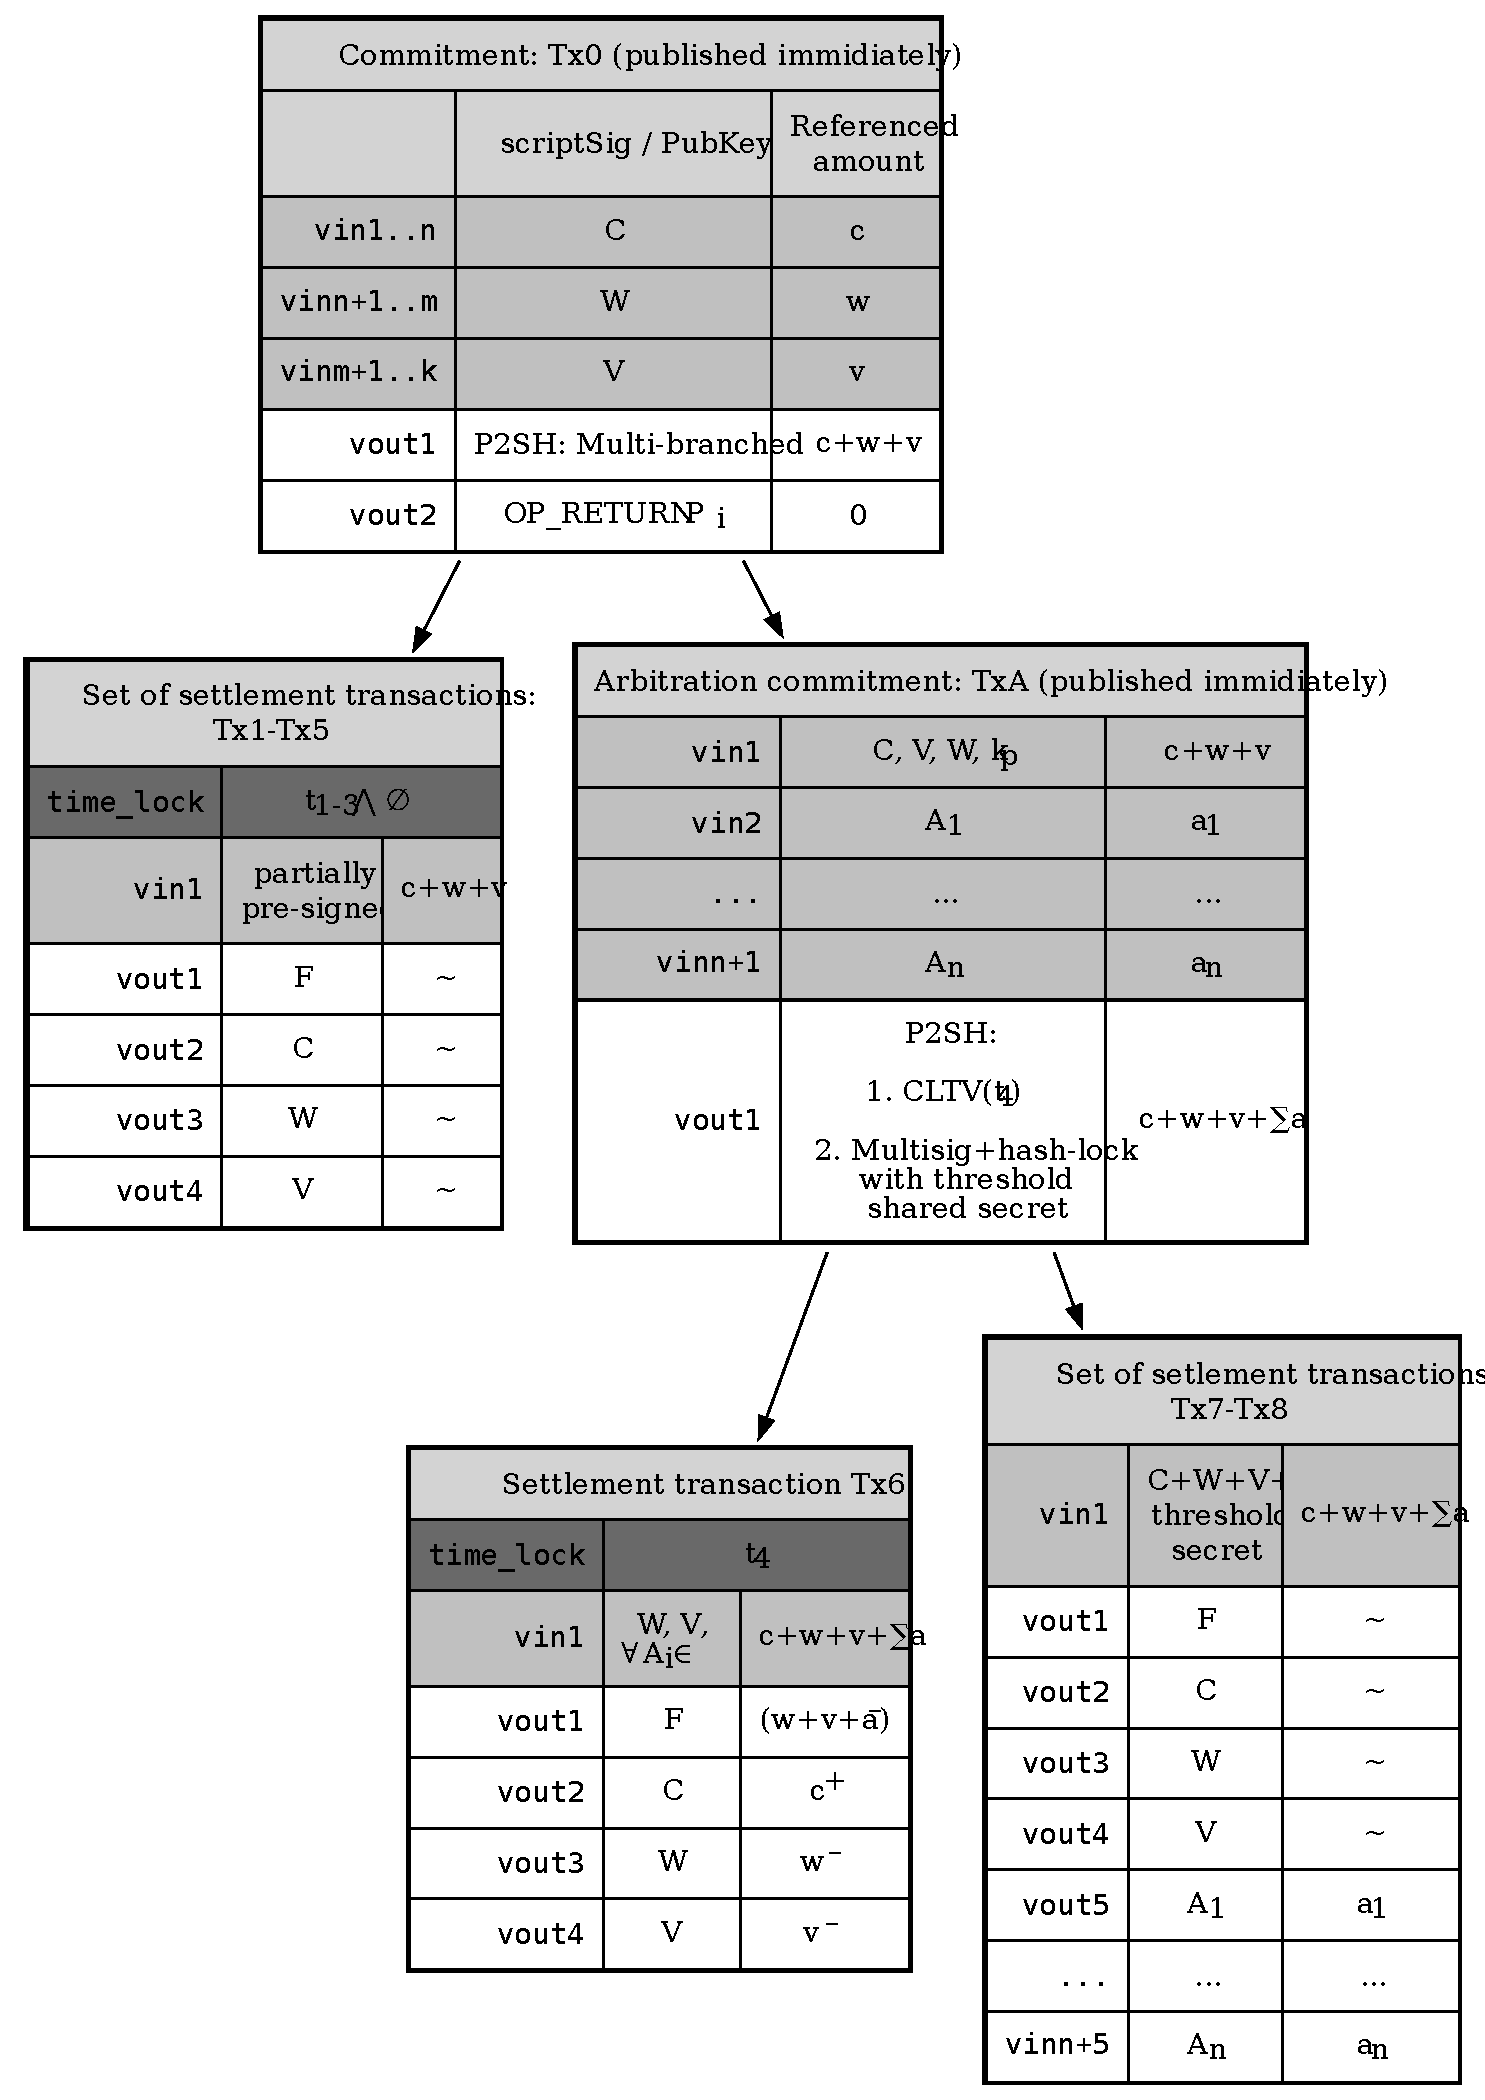
\includegraphics[width=0.9\columnwidth]{assets/txtree.pdf}
    \caption{Details on the structure of the transactions inside $\Upsilon$ transaction tree}
    \caption*{\textit{To be brief, we have simplified some details in the transaction fields:
amounts with superscripts $x^-$ and $x^+$ signify that the recipient will receive  original deposit/stake $x$ either in decreased (slashed) or increased (with some additional payment) form. The exact sizes of the slashes and rewards are provided by the Table~\ref{table:settlement};
\~ tildes stands for "amount might vary", please check the Table~\ref{table:settlement} for specific amounts for different settlement schemes corresponding to the given transaction ids according to the Table~\ref{table:tx}}}
    \label{fig:txtree}
\end{figure}

\subsubsection{Arbitration commitment ceremony}
\label{ceremony}

The ceremony must guarantee:
\begin{enumerate}
    \item Random selection of Arbiters, that were existed before the creation of the \textit{computation contract} and have committed with some stake. This prevents occupation of the network with pre-registered Arbiters and excludes possibility of the participants to change the existing Arbiters depending on the strategy of contract execution.
    \item Commitment from the selected Arbiters to participate in the contract execution.
    \item Absence of censorship from one party or any kind of coalition from the contract participants.
\end{enumerate}

These criteria are satisfied by the following procedure:
\begin{enumerate}
    \item A global set of arbiters $\mathbb{A} \mid \Gamma^\Omega$ is known in global on-chain scope before the initiation of the contract and fixed with a snapshot for the full time of contract execution.
    
    \item All of its participants of $\mathbb{A}$ have committed to the same parameters of the contract (i.e. the same Prometheus contract $\mathsf{P}$) and have locked their stake with a proper \textit{arbitration offer} transaction: $\forall A_i \in \mathbb{A} \mid \mathsf{P}_x: \exists \mathsf{O}_i \mid \Gamma^\Omega = \langle \mathsf{P}_x \dots \rangle$. For details on arbitration offers see the corresponding section in the current chapter.
    
    \item Deterministic random oracle is utilized by all contract participants to sample $\mathbb{A}$. The simplest form of the oracle is a hash function taken from concatenated string of all \texttt{txid} used by $\mathbb{A}$ participants in their arbitration offer transactions.
    
    \item Each of $C, V, W$ does the following in an independent manner:
    \begin{itemize}
        \item Sample set $\mathbb{A}$ in an iterative manner by sending requests to the P2P network and collecting responses of those arbiters who will to participate in the contract. This continues until each of the participants will make a list $\mathcal{A}, |\mathcal{A}|=\mu$ of the parties that have responded to the request.
        
        \item Present to others participants in $\Lambda^\mathsf{S}$ his own view on $\mathcal{A}$, namely $\mathcal{A}^W, \mathcal{A}^V, \mathcal{A}^C$.
        
        \item Compute $\mathcal{A}' = \mathcal{A}^W \cup \mathcal{A}^V \cup \mathcal{A}^C$ and reorder it according to the original random sampling order, select subset $\mathcal{A} \subset \mathcal{A}': \mathcal{A} = \{ A_i \in \mathcal{A}': i \le \mu \}$.
        
        \item Prepare $\mathsf{T^\star_A}$ with all necessary fields (see Fig.~\ref{fig:txtree}) including all of the Arbiters from $\mathcal{A}$ and sign $\mathsf{T^\star_A}$ with each of the $\mathcal{A}$ participants (via P2P communications)
        
        \item Run Shamir's secret sharing protocol extended with collective secret generation procedure as described in \cite{typhon} across all selected arbiters $\mathcal{A}$
    \end{itemize}
    
    \item If there were no Byzantine parties, at the end of this ceremony all of participants will have the same version of $\mathsf{T^\star_A}$. 
    
    \item If the version of $\mathsf{T^\star_A}$ does not match between the participants, the channel and computation contract must be closed via $\Lambda^\mathsf{S} \rightarrow \Lambda^\times$ procedure. The Client may try to set up another computing contract by opening new channel and running the same procedure with different $W$ and $V$.
    
\end{enumerate}

\subsubsection{Completion of channel creation}
Transactions, constituting $\Upsilon$ of \textit{computational contract} $\mathsf{C}$ during the setup phase $\Lambda^\mathsf{S}$ must be (partially)signed in the foolowing order: $\mathsf{T^\star_A} \parallel \mathsf{T^\star_6} \prec \mathsf{T^\star_{7,8}} \prec \mathsf{T^\star_{1\dots 5}} \prec \mathsf{T_0}$. This order is important so that inability to successfully accomplish the arbitration commitment ceremony will result in proper channel termination without option for possible Byzantine parties to publish the rest of prepared transactions on-chain and failure channel closure.

Upon the completion of the $\Upsilon$ construction the original fully-signed \textit{commitment transaction} must be brought into the global space by the Client, putting its last signature upon it. Following publishing of the commitment transaction and its inclusion into the blockchain the transaction becomes \textit{computing contract} as it is seen by everybody in the global on-chain scope $\mathsf{T}_0 \equiv \mathsf{C} \mid \Gamma^\Omega = \langle \mathsf{P}_i, C, W, V, c, w_p, v_p\rangle$ (pls. note that the payload data part of the $\mathsf{C}$ is kept off-chain within the channel scope $\Lambda$, being known only to channel participants). The transaction tree $\Upsilon$ from now till the end of computation and validation stages persists in the state shown on Fig.~\ref{fig:upsilon}.

\begin{figure}[h!]
    \centering
    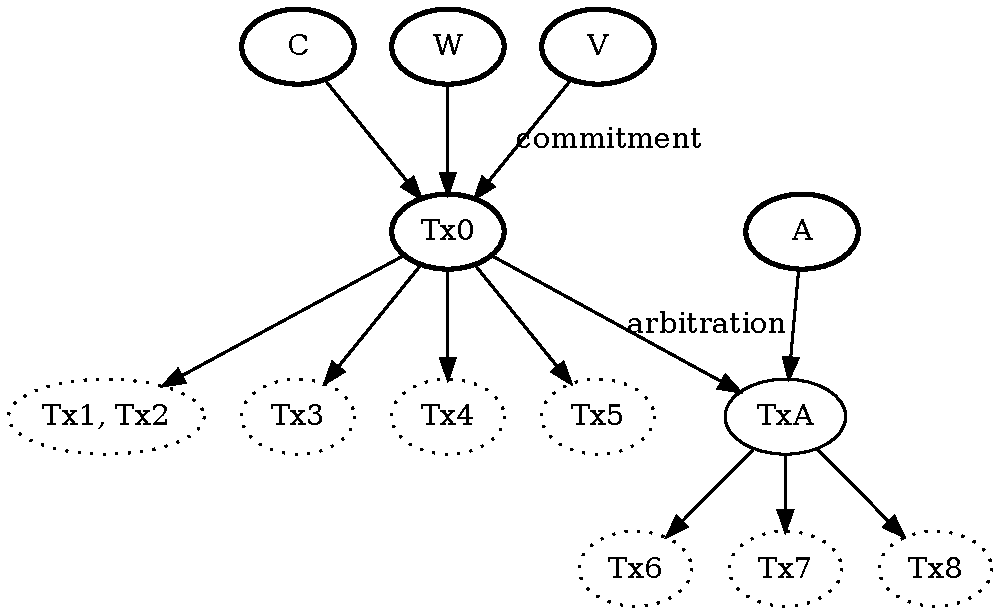
\includegraphics[width=0.75\columnwidth]{assets/upsilon.pdf}
    \caption{Transaction tree $\Upsilon\mid(\Lambda^{\mathsf{C}\vee\mathsf{V}} \cup \Gamma)$ during computation and verification channel states}
    \caption*{\textit{On-chain/published transactions (thus, defined in $\Gamma^\Omega$ scope) are shown in bold, partially-signed transactions -- with dotted line.}}
    \label{fig:upsilon}
\end{figure}

\subsubsection{Normal channel operation and closure}
Prometheus settlement algorithm is implemented utilising partially-signed transactions from the $\Upsilon$ (Fig.~\ref{fig:upsilon}), prepared at the setup phase by all involved parties. They are consist of two subsets: \textit{pre-arbitration} and \textit{post-arbitration transactions}. 

Pre-arbitration transactions are specified in the Table~\ref{table:tx} and Fig.~\ref{fig:txtree}-\ref{fig:upsilon} by their ids \texttt{Tx1-Tx5}. These transactions cover all settlement schemes outside Arbitration and remain unpublished, i.e. residing off-chain in the channel scope as a part of multiparty channel state $\mathsf{T}_{1\dots5} \in \mathsf{M}(\mathsf{C}_i) \mid \Lambda$. Upon corresponding state transitions from the Fig.~\ref{fig:states} they will be signed by the proper party (see "Post-signed" column in the Table~\ref{table:tx}), and published into the global scope to be included on-chain. This completes computing contract $\mathsf{C}$, invalidates local scope $\Lambda$ and closes the state channel $\mathsf{M}(\mathsf{C})$ according to the corresponding settlement scheme from the Table~\ref{table:settlement}:

$(\mathsf{T}^\star_j\mid\Lambda) \xrightarrow{C \vee W \vee V} (\mathsf{T}_j \mid \Gamma^\Omega);\enspace \exists j: 1 \le j \le 5\quad \Longrightarrow \quad \mathsf{M}(\mathsf{C}) \mid (\Lambda^{\mathsf{S}\vee\mathsf{C}\vee\mathsf{V}} \rightarrow \Lambda^\times_{\mathsf{1\dots4}})$

For the settlement schemes that have to reveal computation results to the client (\#2 and \#3), the signing Worker node must additionally include into the signed transaction \textit{preimage} $h_p$ that was originally used for the results encryption. This is required by unlocking script of \texttt{Tx0} which contains hash-lock conditions in branches related to these settlement schemes (see below section on the unlocking scripts details).

\begin{table}[h!]
    \caption{Settlement transactions and their finalisation conditions}
    \label{table:tx}
    \begin{adjustbox}{center}
        \begin{tabular}{@{} r r c c c c @{}}
            \toprule
            Id & Payout Schedule & Pre-signed & Post-signed & Hashlock & nTimelock\\
            \midrule
            \texttt{Tx1} & \#1   & $W, C$ & $V$ & - & $t_3$ \\
            \texttt{Tx2} & \#1   & $W, V$ & $C$ & - & $t_3$ \\
            \texttt{Tx3} & \#2   & $V, C$ & $W$ & $h_p$ & $t_2$ \\
            \texttt{Tx4} & \#3   & $C, W$ & $V$ & $h_p$ & - \\
            \texttt{Tx5} & \#4   & $C, W$ & $V$ & - & $t_1$ \\
            \texttt{TxA} & \#5-7 & $C, W, A$ & $V$ & $k_p$ & - \\
            \texttt{Tx6} & \#5   & $V, W, A$ & $C$ & - & $t_4$ \\
            \texttt{Tx7} & \#6   & $C, W, V$ & - & $T^k_n(\mathcal{A^+})$ & - \\
            \texttt{Tx8} & \#7   & $C, W, V$ & - & $T^k_n(\mathcal{A^+})$, $h_p$ & w \\
            \bottomrule
        \end{tabular}
    \end{adjustbox}
\end{table}

\subsubsection{Arbitration}

In order to transition the channel state into the Arbitration, $\mathsf{M}(\mathsf{C}) \mid \Lambda^{\mathsf{C}} \rightarrow \Lambda^{\mathsf{A}}$, Worker must submit appeal by including its \textit{arbitration-unlocking preimage} $k_p$ into \texttt{scriptSig} of \texttt{TxA} (which is already signed by the Verifier as part of its \textit{verdict} on the Worker fault) and publishing the transaction:

$(\mathsf{T}^\star_A\mid\Lambda^\mathsf{V}) \xrightarrow{k_p} (\mathsf{T}_A\mid\Gamma^\Omega) \quad \Longrightarrow \quad\mathsf{M}(\mathsf{C}) \mid (\Lambda^{\mathsf{V}} \xrightarrow{\mathtt{appeal}} \Lambda^{\mathsf{A}})$.

This signals to the arbiters in $\mathcal{A}$ to initiate their verification procedure on the data from $\mathsf{M}$, mainly PCP proofs $\pi$.

Arbitration is completed in one of the ways defined in the previous chapter. Each of them has a corresponding pre-signed transaction \texttt{Tx6-8} (Table~\ref{table:tx}), which can be finalised by the interested party and published into the global scope, which will close the channel and complete settlement:

$(\mathsf{T}^\star_j\mid\Lambda) \xrightarrow{C \vee \mathcal{A}^+} (\mathsf{T}_j \mid \Gamma^\Omega);\enspace \exists j: 6 \le j \le 8\quad \Longrightarrow \quad \mathsf{M}(\mathsf{C}) \mid (\Lambda^{\mathsf{A}} \rightarrow \Lambda^\times_{\mathsf{5\dots7}})$

Arbiters that came to the \textit{coherent decision} sign transactions \texttt{Tx7-Tx8} by revealing their parts of the collectively shared secret with a threshold signature $T^k_n$, the corresponding revealed secret is a \textit{preimage} for the hashlock condition in \texttt{scriptSig} part of the transactions.

\section{Conclusion}

In the present work we have formally defined Prometheus: a protocol for running high-load \& machine learning computing inside a trustless decentralized environment in Byzantine-tolerant way, utilizing zero knowledge  computation integrity arguments, economic incentives and p2p networking. The paper have covered protocol design rationale, architecture, formal protocol definition and specified protocol operations with demonstrable Nash equilibrium, as well as transaction model for implementation with Bitcoin blockchain and script functionality.

\nocite{*}
\bibliographystyle{abbrv}
\bibliography{references}

\end{document}
